\chapter{Operador de Cruza}

Los operadores de cruza permiten generar nuevos individuos (hijos) a partir de dos padres, combinando partes de sus cromosomas. A continuación se describen distintos métodos de cruza utilizados en algoritmos evolutivos.

\section{One Point}

Dados dos padres $p_1$ y $p_2$ con cromosomas de tamaño $T$, se selecciona una posición al azar $t \in [1, T-1]$ donde se particionan y combinan los genes:
\begin{gather*}
	h_1 = [0, t)_{p_1} \cup [t, T)_{p_2} \\
	h_2 = [0, t)_{p_2} \cup [t, T)_{p_1}
\end{gather*}

Tal como se muestra en la figura \ref{fig:cross_one}, con $t = 3$.

\begin{figure}[H]
	\centering
	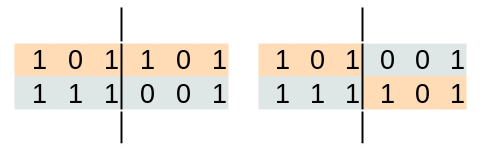
\includegraphics[width=0.75\linewidth]{img/cross_one.png}
	\caption{Ejemplo de cruza en un solo punto}
	\label{fig:cross_one}
\end{figure}

\section{Two Point}

Tiene un comportamiento similar al anterior. Dados dos padres $p_1$ y $p_2$ con cromosomas de tamaño $T$, se seleccionan dos posiciones al azar $t_1, t_2$ tales que $0 \leq t_1 < t_2 \leq T$. Se intercambia el segmento entre ambas posiciones:
\begin{gather*}
	h_1 = [0, t_1)_{p_1} \cup [t_1, t_2)_{p_2} \cup [t_2, T)_{p_1} \\
	h_2 = [0, t_1)_{p_2} \cup [t_1, t_2)_{p_1} \cup [t_2, T)_{p_2}
\end{gather*}

\begin{figure}[H]
	\centering
	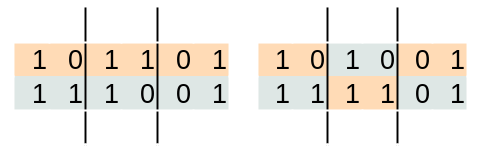
\includegraphics[width=0.75\linewidth]{img/cross_two.png}
	\caption{Ejemplo de cruza en dos puntos}
	\label{fig:cross_two}
\end{figure}

\section{Uniform}

Dados dos padres $p_1$ y $p_2$ con cromosomas de tamaño $T$, se genera una máscara binaria aleatoria $M \in \{0, 1\}^T$. Si $M[i] = 0$, entonces $h_1[i] = p_1[i]$ y $h_2[i] = p_2[i]$; si $M[i] = 1$, entonces $h_1[i] = p_2[i]$ y $h_2[i] = p_1[i]$.

\begin{figure}[H]
	\centering
	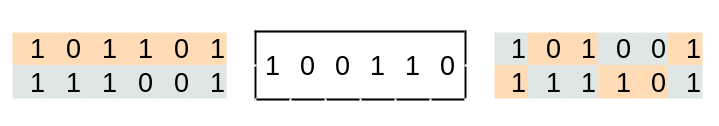
\includegraphics[width=0.75\linewidth]{img/cross_uniform.png}
	\caption{Ejemplo de cruza uniforme}
	\label{fig:cross_uniform}
\end{figure}

\section{Arithmetic}

Para cada par de padres, se genera un valor aleatorio $\alpha \in [0, 1]$ que define una combinación lineal entre sus genes. Para cada posición $i$ del cromosoma:
\begin{gather*}
	h_1[i] = \alpha \cdot p_1[i] + (1 - \alpha) \cdot p_2[i] \\
	h_2[i] = (1 - \alpha) \cdot p_1[i] + \alpha \cdot p_2[i]
\end{gather*}

Este operador es común en representaciones reales y mantiene los genes dentro del espacio de búsqueda.

\section{Blend (BLX-$\alpha$)}

El operador \textit{Blend Crossover} permite generar valores fuera del intervalo definido por los padres. Para cada gen $i$ se define un intervalo extendido:

\[
\text{min}_i = \min(p_1[i], p_2[i]), \quad
\text{max}_i = \max(p_1[i], p_2[i])
\]

El hijo se genera como:
\[
h[i] = U\left( \text{min}_i - d, \text{max}_i + d \right)
\quad \text{donde } d = \alpha \cdot (\text{max}_i - \text{min}_i)
\]

El parámetro $\alpha$ controla cuánto se puede explorar fuera del rango original. La función $U$ es la función de distribución uniforme continua.

\section{Simulated Binary (SBX)}

El operador \textit{Simulated Binary Crossover} simula el comportamiento del cruce de un solo punto en cromosomas reales. Dado un parámetro de distribución $\eta$, se calcula un factor $\beta$ basado en una variable aleatoria $u \sim U(0,1)$:

\[
\beta = \begin{cases}
	(2u)^{1/(\eta + 1)} & \text{si } u \leq 0.5 \\
	\left( \frac{1}{2(1 - u)} \right)^{1/(\eta + 1)} & \text{si } u > 0.5
\end{cases}
\]

Entonces, los hijos se calculan como:
\begin{gather*}
	h_1[i] = 0.5 \cdot \left( (1 + \beta) \cdot p_1[i] + (1 - \beta) \cdot p_2[i] \right) \\
	h_2[i] = 0.5 \cdot \left( (1 - \beta) \cdot p_1[i] + (1 + \beta) \cdot p_2[i] \right)
\end{gather*}

\section{Uniform Order Based}

Este operador está diseñado para cromosomas con permutaciones (como en el problema del viajante). Se genera una máscara binaria $M$ de tamaño $T$. Las posiciones con 1 se copian directamente del primer padre al hijo. Las posiciones con 0 se rellenan, en orden, con los genes del segundo padre que no estén ya presentes en el hijo.

Este método mantiene la posición relativa y evita duplicados.

\section{Order Based}

También usado en permutaciones. Se seleccionan $k$ posiciones aleatorias del primer padre y se copian al hijo. Luego, se rellena el resto del hijo con los genes del segundo padre manteniendo el orden relativo y omitiendo duplicados.

Este operador es útil cuando el orden de los elementos en el cromosoma es relevante, como en rutas o secuencias.

\begin{table}[H]
	\centering
	\begin{tabular}{|l|c|c|}
		\hline
		\textbf{Operador de Cruza} & \textbf{Espacio que abarca} & \textbf{Representación}  \\ \hline
		One Point                  & Local                        & Binaria             \\ \hline
		Two Point                 & Local                        & Binaria             \\ \hline
		Uniform                   & Moderado                     & Binaria       \\ \hline
		Arithmetic                & Local                        & Real                 \\ \hline
		Blend (BLX-$\alpha$)       & Global (controlado por $\alpha$) & Real\\ \hline
		Simulated Binary (SBX)     & Global (controlado por $\eta$) & Real   \\ \hline
		Uniform Order Based       & Moderado                     & Permutacional    \\ \hline
		Order Based               & Moderado                     & Permutacional           \\ \hline
	\end{tabular}
	\caption{Comparativa de operadores de cruza según el tipo de representación y cobertura del espacio de búsqueda.}
	\label{tab:cross_comparison}
\end{table}

